\section{Spread impact}\label{sec:spread_impact}

When we calculate the price response functions, the signal of the response depends
directly on the analyzed stock. Thus, even if the responses functions are in
the same scale, their values differ from one to another. We choose the spread
to group 530 stocks in the NASDAQ stock market for the year 2008, and check if
the average strength of the price self-response functions in physical time scale were
similar for this groups. For each stock we computed the average spread for a
year, and using this value we classified the groups.

We used five intervals to select the stocks groups to average the response
functions ($s<0.03\$$, $0.03\$ \le s <0.06\$$, $0.06\$ \le s <0.09\$$,
$0.09\$ \le s <0.15\$$, $s \ge 0.15\$$). The detailed information of the groups
can be seen in Appendix \ref{app:spread_impact}.

In Fig. \ref{fig:spread_impact} can be seen the average response functions for
the five groups. The response functions start at the bottom with the average
response for the stocks with the smaller spreads (more liquid) and grow to the
larger average response functions for the stocks with the larger spreads (less
liquid). All the average response functions follows the increment to a maximum
followed by a decrease described in Sect. \ref{sec:response_functions_def} and
\ref{sec:response_functions_imp}.

\begin{figure}[htbp]
    \centering
    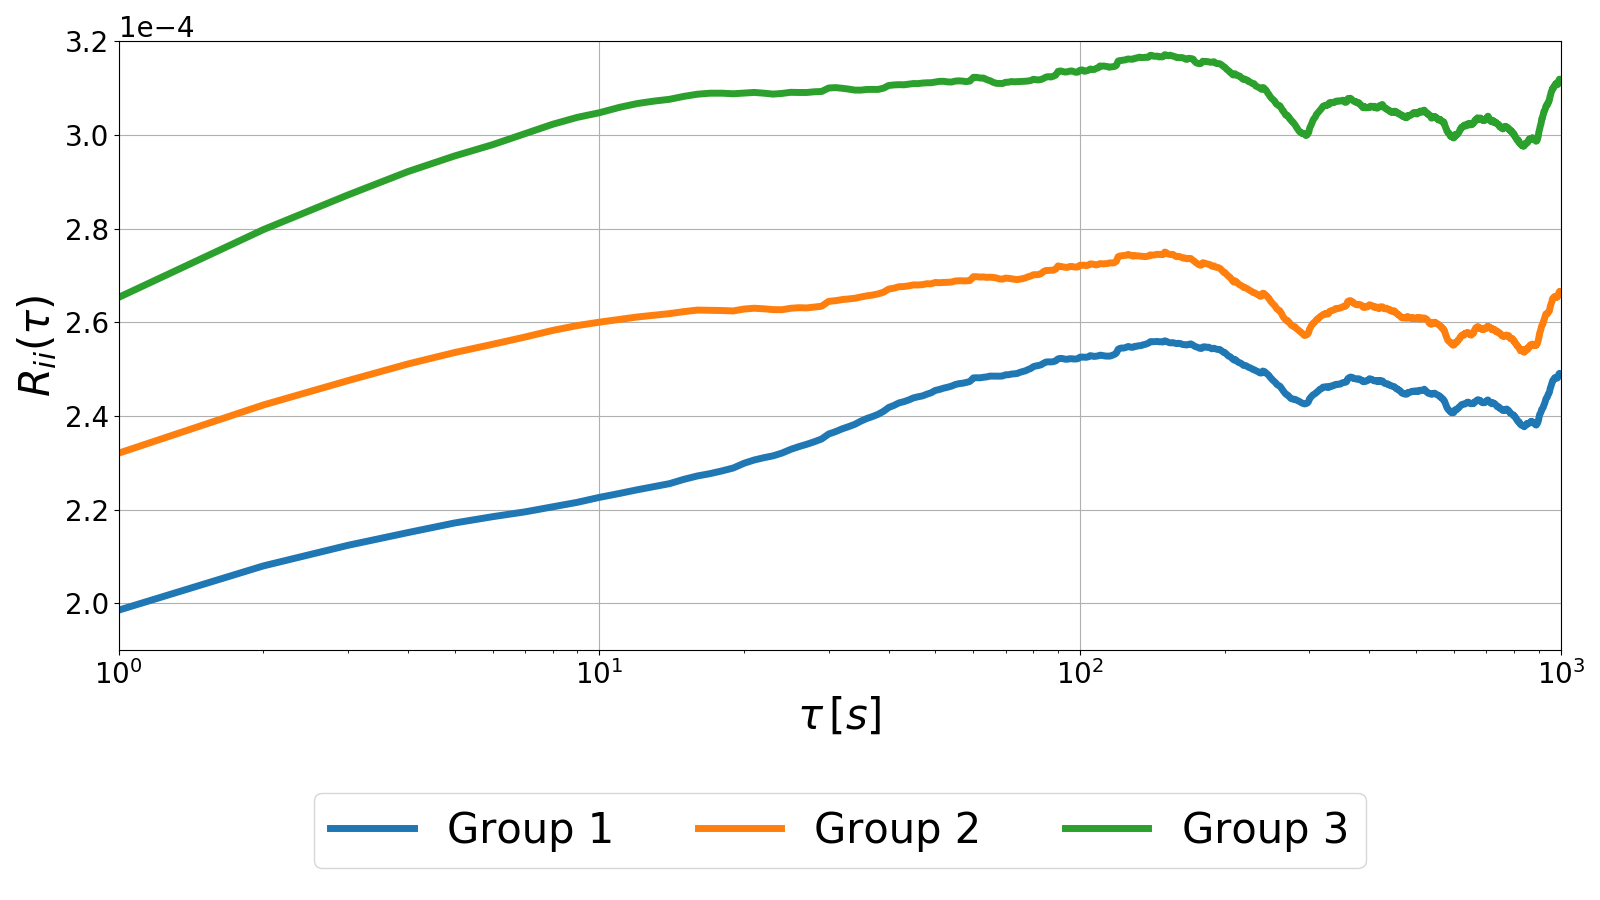
\includegraphics[width=\columnwidth]{figures/06_spread_impact_2008.png}
    \caption{Average price self-response functions
             $R^{p}_{ii}\left(\tau\right)$ excluding
             $\varepsilon^{p}_{i}\left(t\right) = 0$ in 2008 versus time lag
             $\tau$ on a logarithmic scale in physical time scale for 530
             stocks divided in three representative groups.}
    \label{fig:spread_impact}
\end{figure}

The strength of the self-response function signals grouped by spread can be
explained knowing that the response functions directly depend on trade signs.
As long as the stock is liquid, the number of trade signs grow. Thus, at the
moment of the averaging, the large amount of trades, reduces the response
function signal. Therefore, the response function decrease as long as the
liquidity grows. And as stated in the introduction the spread is negatively
related to trading volume, hence, firms with more liquidity tend to have lower
spreads.
